\documentclass[preprint,12pt]{elsarticle}

\usepackage{amsmath,amssymb,booktabs,graphicx}
\usepackage[version=4]{mhchem}
\journal{Nuclear Engineering and Technology}

\begin{document}
\begin{frontmatter}

\title{A Modular Physics-Informed Surrogate-Based Framework for Multi-Objective Optimization of Multilayer Radiation Shields under Geometric Constraints}

\author[pen]{Jo\~ao Vitor Mendes da Silva}
\author[ime]{Wallace Vallory Nunes}
\author[ime]{Marcos Paulo Cavaliere}
\author[pen]{Inay\'a Corr\^ea Barbosa Lima}
\affiliation[ime]{organization={Military Institute of Engineering (IME)},
 addressline={Pra\c{c}a General Tib\'urcio, 80, Urca}, city={Rio de Janeiro}, postcode={22290-270}, country={Brazil}}
\affiliation[pen]{organization={Nuclear Engineering Program (PEN/COPPE), Federal University of Rio de Janeiro (UFRJ)},
 addressline={Av. Hor\'acio Macedo, 2030, Cidade Universit\'aria}, city={Rio de Janeiro}, postcode={21941-972}, country={Brazil}}

\begin{abstract}
Multilayer radiation-shielding optimization is characterized by high-dimensional design spaces, computationally expensive evaluations, and conflicting objective functions. This study proposes SPHIN (Sobol-PHysics-Informed NSGA-II), a modular framework for multi-objective optimization of multilayer radiation shields with respect to effective dose, weight, and material cost. SPHIN combines scrambled Sobol sampling with a feasibility-adjustment method (FAM), automated MCNP6 transport simulations, physics-informed surrogate modeling, and an adaptive NSGA-II followed by TOPSIS-IQR as a compromise-selection rule. The case study is a seven-layer semi-cylindrical shield exposed to a 3.7 TBq \ce{^{60}Co} source. The 2,000-case MCNP6 campaign used an F4:P tally with energy-dependent DE4/DF4 effective-dose coefficients for anterior--posterior irradiation from ICRP Publication 116. The campaign covers effective doses from 18.728 to 33.858 mSv per 5 min. The selected Elastic Net surrogate achieved a held-out test-set $R^2$ of 0.9870 after selection exclusively by mean five-fold cross-validation $R^2$ on the training data. In ten paired seeds, the adaptive NSGA-II obtained higher fixed-reference hypervolume than the canonical implementation in seven runs (paired Wilcoxon $p=0.0273$) and lower generalized spread ($p=0.0020$) for this case study. Independent MCNP6 validation of 21 pre-specified Pareto solutions yielded a mean absolute percentage error of 4.33\%. The resulting architecture is modular and applicable to shielding-design problems in which high-fidelity radiation transport is expensive.
\end{abstract}

\begin{keyword}
Sobol sequences \sep MCNP6 \sep Machine learning \sep Multi-objective optimization \sep NSGA-II \sep Radiation shielding \sep Surrogate modeling
\end{keyword}
\end{frontmatter}

\section*{Highlights}
\begin{itemize}
\item Scrambled Sobol+FAM improved grid coverage by 4.5\% and mean nearest-neighbor distance by 4.2\% relative to random+FAM.
\item MCNP6 effective dose was scored with an F4:P tally and energy-dependent ICRP 116 AP coefficients.
\item Elastic Net was selected using training-set five-fold cross-validation; the test set was reserved for final reporting.
\item Adaptive and canonical NSGA-II were compared in ten paired random seeds using fixed-reference metrics.
\item Twenty-one pre-specified Pareto solutions were independently validated with MCNP6.
\end{itemize}

\section{Introduction}
Radiation shielding provides a passive barrier against exposure to ionizing radiation in stationary facilities, medical environments, mobile platforms, and emergency-response scenarios. Shield design affects regulatory compliance, system cost, and operation \citep{Shultis2016}.

Optimization plays a central role in nuclear-engineering design \citep{Price2022}. Shielding design is multi-objective, particularly when global geometry is fixed and the optimization concerns material selection, ordering, and layer-thickness allocation \citep{Bagheri2023,Liu2026}. Even a seven-layer shield generates a large mixed discrete--continuous design space. Direct evaluation with high-fidelity Monte Carlo N-Particle (MCNP) transport calculations is consequently expensive \citep{Werner2017}.

When the available high-fidelity budget is limited, the sampling scheme is itself a modeling decision. Scrambled Sobol sequences provide a reproducible low-discrepancy alternative to purely random sampling \citep{Sobol1967,Owen1997,JoeKuo2008}; however, their practical advantage depends on the problem's effective dimension and on transformations imposed by feasibility constraints \citep{Kucherenko2011,Renardy2021}. This distinction is consequential here because thicknesses must lie on a bounded fixed-sum simplex. Accordingly, the present design treats the final Sobol+FAM sample as an operational quasi-random design and reports diagnostics of the transformed configurations, rather than asserting ideal Sobol-net properties after projection.

Surrogate-assisted evolutionary optimization is a suitable response to the transport-computation bottleneck \citep{Jin2011,Erdem2025}. Physics-informed machine learning can incorporate prior physical structure to improve data efficiency and interpretability, while still requiring empirical validation in the application domain \citep{Karniadakis2021}. In the present study, this principle is implemented through transparent configuration descriptors, not through a claim that the surrogate enforces the transport equation. Recent radiation-shielding studies have combined transport calculations, learned predictors, and evolutionary optimization \citep{Song2021,Gui2025,He2025,Chowdhury2026}; they motivate, but do not remove, the need for a reproducible comparison and independent transport validation.

Generic optimization environments such as NEORL demonstrate the value of modular software for mixed and constrained engineering problems \citep{Radaideh2023}. Nevertheless, a shielding workflow must also make explicit the design generation, transport-to-dose conversion, physical feature construction, surrogate-selection protocol, and post-optimization validation. Four scoped gaps therefore motivate SPHIN: (i) feasible, diagnostically characterized sampling rather than unconstrained random designs; (ii) interpretable physics-guided descriptors alongside raw configuration variables; (iii) a modular path from MCNP6 data to a surrogate-assisted multi-objective search with a canonical baseline; and (iv) a compromise-selection rule whose normalization and weights are subjected to sensitivity analysis.

This work introduces SPHIN (Sobol-PHysics-Informed NSGA-II), a systematic and modular workflow comprising: (i) scrambled Sobol sampling with feasibility restoration; (ii) automated MCNP6 simulations; (iii) surrogate modeling with physics-informed and heuristic-guided features; and (iv) adaptive NSGA-II optimization and TOPSIS-IQR compromise selection. The framework is demonstrated for a seven-layer semi-cylindrical shield under \ce{^{60}Co} gamma irradiation, simultaneously minimizing effective dose, shield weight, and material cost. Its architecture is designed so that the sampling, radiation field, geometry, transport code, surrogate, or optimizer can be replaced, provided that the high-fidelity dataset and validation are regenerated for the new domain.

\section{The SPHIN Framework}
SPHIN addresses high dimensionality, costly simulations, and conflicting objectives through the modular architecture shown in Figure~\ref{fig:framework}. Its modules exchange standardized configuration and result files, so that the sampling, transport, surrogate, or optimization component can be replaced without changing the overall workflow.

\begin{figure}[htbp]
\centering
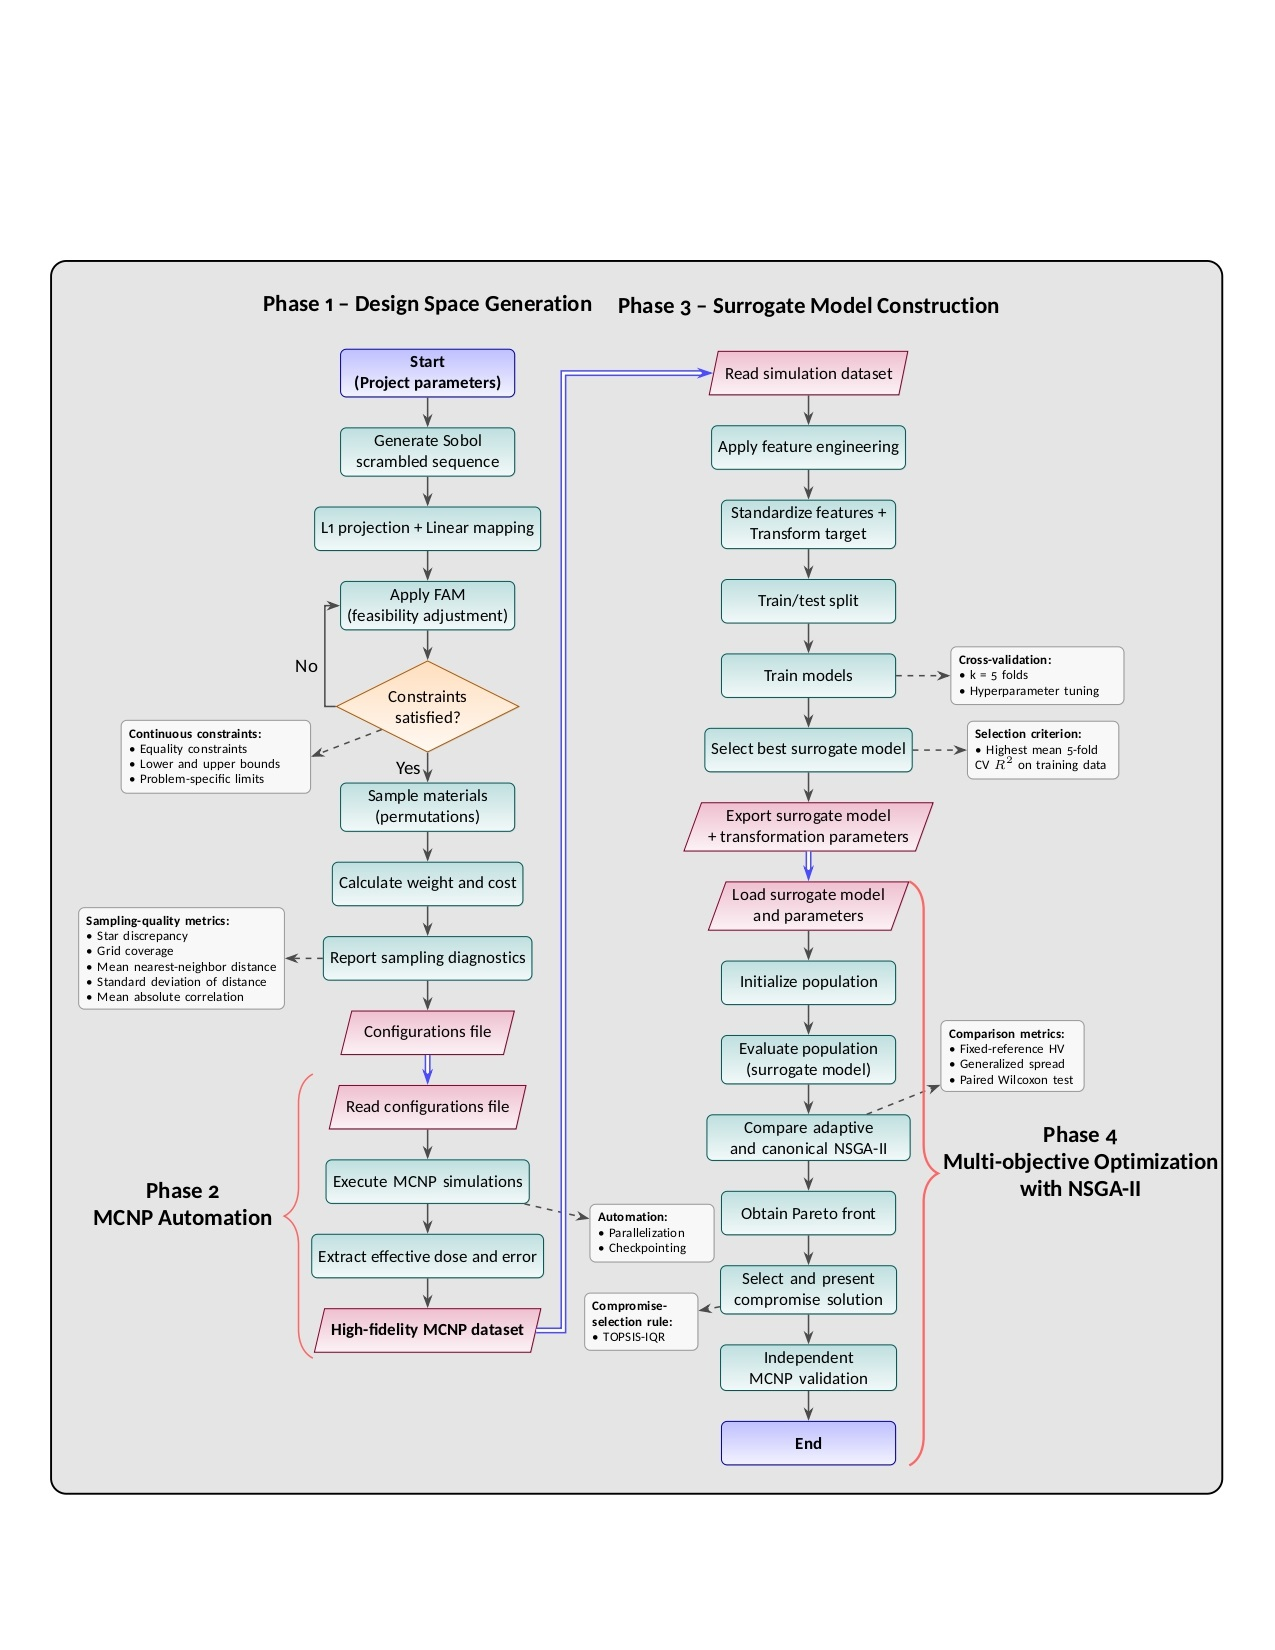
\includegraphics[width=\linewidth]{figures/fig1_framework.jpg}
\caption{SPHIN framework architecture: systematic sampling, high-fidelity MCNP6 transport calculation, surrogate modeling, multi-objective optimization, and independent validation.}
\label{fig:framework}
\end{figure}

\subsection{Phase 1: Systematic design-space generation}
The design vector contains seven continuous layer thicknesses and seven categorical material assignments. The continuous constraints are a fixed total shielding thickness of 6.0 cm and individual bounds of 0.2--2.0 cm. The discrete constraint requires all seven selected candidate materials to be distinct in each configuration.

A total of $N=2000$ points were generated with scrambled Sobol sequences \citep{Owen1997}, implemented with \emph{scipy.stats.qmc.Sobol} \citep{Virtanen2020} using \emph{scramble=True} and seed 123. The samples were L1-projected and linearly mapped to layer thicknesses. The feasibility-adjustment method (FAM) then clips any layer above 2.0 cm and redistributes its excess thickness among the remaining layers according to their available margins. It therefore restores only the continuous thickness constraints; random permutations subsequently assign the seven distinct materials. FAM converged for all configurations in at most two iterations.

Sampling diagnostics are reported using five metrics: star discrepancy, grid coverage, mean nearest-neighbor distance, standard deviation of nearest-neighbor distance, and mean absolute inter-variable correlation. They characterize the operational quasi-random sample after projection and FAM, rather than claiming that it remains an ideal Sobol net on the simplex. In particular, $N=2000$ is not a power of two and L1 projection changes the distribution induced by the original Sobol points; the resulting sample is therefore described as an operational quasi-random design.

Because the seven candidate materials are required to be distinct and there are seven layers, every configuration contains each candidate material exactly once. The 2,000 configurations cover 39.7\% of the $7!=5040$ possible material orders, sampled without replacement using the fixed generation seed. This is a purposeful case-study restriction, including the mandatory presence of B$_4$C--HDPE, rather than an exhaustive optimization over arbitrary material compositions.

\subsection{Phase 2: Automated MCNP6 simulations}
For each feasible configuration, a parameterized MCNP6 input was generated for the geometry in Section~\ref{sec:problem}. The source--detector center distance was 121 cm. The campaign comprised 2,000 simulations with $1\times10^8$ particle histories per case.

Effective dose was evaluated with an F4:P cell-flux tally coupled to the energy-dependent DE4/DF4 fluence-to-effective-dose coefficients for anterior--posterior irradiation from ICRP Publication 116 \citep{ICRP116}. The FM4 multiplier was 7400, accounting for the source activity (3.7 TBq), two photons per \ce{^{60}Co} decay, and conversion from pSv to mSv. Unlike a single energy conversion factor, DE4/DF4 accounts for the shield-dependent scattered photon spectrum. Dose, relative error, and tally fluctuation-chart diagnostics were parsed from each output file.

As an independent scale check, the no-shield MCNP6 baseline at 121 cm was 0.215620 mSv/s (64.686 mSv per 5 min), compared with 64.758 mSv per 5 min from a gamma-constant calculation interpolated for the two principal \ce{^{60}Co} photon energies using ICRP nuclear-decay data \citep{ICRP107}, a discrepancy of $-0.112\%$. The corrected shielded campaign produced 18.728--33.858 mSv per 5 min. These values refer to the radiological-only geometry: no grenade component was included.

\subsection{Phase 3: Hybrid feature engineering and surrogate modeling}
The response variable was the effective dose in mSv per 5 min. Sixteen hybrid descriptors combining physical, shielding-strategy, nonlinear-interaction, and material-composition information were derived a priori. The linear attenuation coefficients used in the attenuation-based descriptors correspond to 1.25 MeV and were compiled from NIST XCOM photon cross sections \citep{XCOM}. The sequence score remains a heuristic descriptor of material order; it is not a calibrated transport model. This distinction preserves the physical motivation of the feature set without representing empirical ordering preferences as a calibrated radiation-transport law.

\begin{table}[htbp]
\centering\small
\caption{Hybrid features retained in the surrogate-modeling stage. Physical and composition features are calculated from the candidate layer configuration; the sequence score is heuristic-guided.}
\label{tab:features}
\begin{tabular}{lll}
\toprule
Group & Feature & Characterization\\
\midrule
Physical fundamentals & Weighted effective atomic number; total attenuation; total electron thickness; total transmission & Physics-derived\\
Shielding strategies & High-$Z$ protection; low-$Z$ moderation; high-$Z$/low-$Z$ ratio & Physics-guided\\
Shielding strategies & Sequence score & Heuristic-guided\\
Nonlinear interactions & $Z\times$attenuation interaction & Physics-guided\\
Material composition & Thickness assigned to each material & Direct configuration descriptor\\
\bottomrule
\end{tabular}
\end{table}

The 2,000 simulations were partitioned into 1,700 training and 300 held-out test configurations using a shuffled 85/15 split. The seven layer-material labels were one-hot encoded, yielding 49 binary material features in addition to the seven thicknesses and 16 hybrid descriptors. All transformations and feature scaling were fitted using training data only. Standard scaling was applied to the common feature matrix; the Bayesian Ridge pipeline separately applied degree-two polynomial expansion followed by robust scaling. Candidate models were implemented with scikit-learn \citep{Pedregosa2011} and drawn from regularized-linear \citep{MacKay1992,Zou2005,Wold2001}, tree-based \citep{Breiman2001,Friedman2001,ChenGuestrin2016,Ke2017}, neural-network, and stacking \citep{Wolpert1992} classes. Model selection was performed exclusively on the training data: mean five-fold cross-validation $R^2$ determined the selected model. The Friedman--Nemenyi comparison \citep{Demsar2006} was retained only as an exploratory diagnostic because cross-validation folds are not independent datasets; it was not used to select by test-set performance. The held-out test set was used only for final performance reporting.

\begin{table}[htbp]
\centering\small
\caption{Main optimized model configurations retained from the surrogate-modeling workflow.}
\label{tab:hyperparameters}
\begin{tabular}{p{3.2cm}p{8.0cm}}
\toprule
Model & Main configuration\\
\midrule
Bayesian Ridge (polynomial) & degree=2; RobustScaler; max\_iter=1000; default Bayesian priors\\
Elastic Net & alpha=0.0005; l1\_ratio=0.5; max\_iter=10000; selection=random\\
PLS & n\_components=8; max\_iter=2000\\
Gradient Boosting & 800 estimators; learning rate 0.008; depth 5; subsampling 0.7\\
Random Forest & 400 estimators; depth 12; feature fraction 0.7\\
XGBoost & 700 estimators; learning rate 0.01; subsampling and column sampling 0.75\\
HistGradientBoosting & 400 iterations; learning rate 0.05; depth 6\\
\bottomrule
\end{tabular}
\end{table}

For computational context, the 2,000-case MCNP6 campaign consumed 14 h with three concurrent jobs, corresponding to an average wall-clock time of 75.6 s per case. On the local evaluation host, the selected Elastic Net required a median 0.292 ms for one 72-feature prediction over five batches of 1,000 calls; the PLS benchmark required 0.399 ms under the same protocol. The corresponding model-only speedup for the selected surrogate is therefore approximately $2.59\times10^{5}$ relative to one MCNP6 case. This is a hardware- and implementation-specific timing comparison; it excludes feature preparation and the analytical objectives used by the optimizer.

\subsection{Phase 4: NSGA-II and compromise selection}
The optimization engine, implemented with DEAP \citep{Fortin2012}, uses population 500 and 300 generations. NSGA-II was selected because it remains a well-established method for constrained multi-objective engineering problems with a small number of objectives \citep{Deb2002,DebJain2014}. Effective dose is predicted by the selected surrogate, while shield weight and material cost are evaluated analytically. Deterministic repair normalizes thicknesses to 6.0 cm, enforces the 0.2--2.0 cm bounds, and makes material assignments distinct.

The adaptive variant modulates mutation according to optimization progress and population diversity and restarts a fraction of poor individuals after stagnation. Its performance was assessed against a canonical NSGA-II under identical settings and ten paired random seeds. Hypervolume was calculated with one fixed global reference point, $(37.24347\ \mathrm{mSv/5\ min}, 264.2563\ \mathrm{kg}, 17593.334\ \mathrm{USD})$, derived before the run comparison. Diversity was measured by generalized spread, which is appropriate for three objectives \citep{Zhou2006}. A two-sided paired Wilcoxon signed-rank test compares both variants across seeds.

For the adaptive variant, the base mutation rate decreases linearly from 0.25 to 0.10 over the $T=300$ generations,
\begin{equation}
p_m(g)=0.25-(0.25-0.10)\frac{g}{T}.
\label{eq:mutation-rate}
\end{equation}
When generalized spread is below 0.3, this rate is multiplied by 1.5 and is clipped to the interval $[0.05,0.50]$. The Gaussian perturbation standard deviation for continuous variables is
\begin{equation}
\sigma(g)=0.15(t_{\max}-t_{\min})\left(1-0.7\frac{g}{T}\right).
\label{eq:mutation-strength}
\end{equation}
After eight generations without a $0.1\%$ hypervolume improvement, the adaptive variant replaces 20\% of the population using feasible random individuals, preserving the remaining rank- and crowding-preferred solutions.

TOPSIS-IQR is used as a compromise-selection rule with equal objective weights, following the TOPSIS ranking concept \citep{HwangYoon1981}. Its IQR normalization reduces sensitivity to extreme objective values, but it is not claimed to be universally superior to min--max or vector normalization. The dependence of the selected compromise on normalization and weights is examined as a sensitivity analysis.

\subsection{Optimization problem description}\label{sec:problem}
The demonstration problem is a seven-layer semi-cylindrical shield exposed to gamma radiation from a 3.7 TBq \ce{^{60}Co} source. The shield has an inner radius of 35 cm, height of 70 cm, and fixed radial thickness of 6 cm. The detector is a cylinder of radius 5 cm and height 10 cm placed at the centre of curvature, 35 cm from the inner shield surface along the source--detector axis. The external source faces the shield outermost layer; the detector faces the innermost layer, as illustrated in Figure~\ref{fig:geometry}.

\begin{figure}[htbp]
\centering
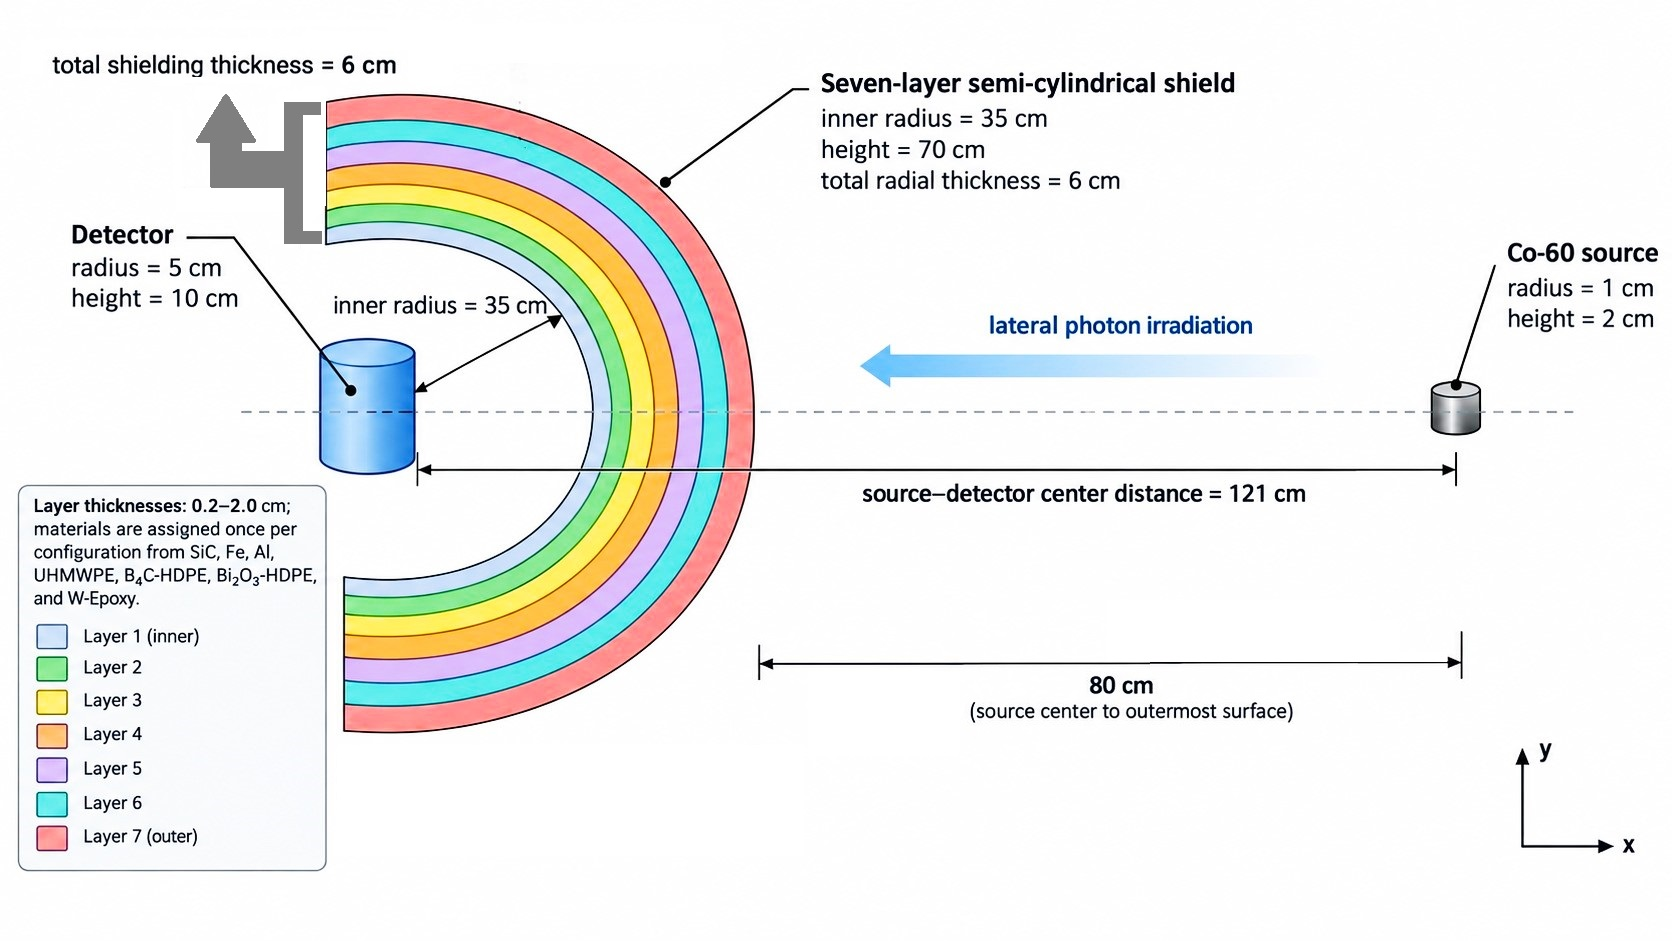
\includegraphics[width=0.95\linewidth]{figures/fig2_geometry.jpg}
\caption{Geometric scenario for the SPHIN case study. The \ce{^{60}Co} source is positioned outside the multilayer semi-cylindrical shield, whereas the detector is at its centre of curvature and faces the innermost layer. The source--detector centre distance is 121 cm.}
\label{fig:geometry}
\end{figure}

\begin{table}[htbp]
\centering
\caption{Candidate shielding materials.}
\label{tab:materials}
\begin{tabular}{llll}
\toprule
Material & Composition & Density (g/cm$^3$) & Cost (USD/kg)\\
\midrule
SiC & Silicon carbide & 3.21 & 0.90\\
Fe & Rebar HRB400E & 7.87 & 0.46\\
Al & Aluminum A00 & 2.70 & 3.38\\
UHMWPE & $(\mathrm{C_2H_4})_n$ & 0.96 & 1.33\\
B$_4$C--HDPE & 30 vol.\% B$_4$C + 70 vol.\% HDPE & 1.43 & 6.55\\
Bi$_2$O$_3$--HDPE & 70 wt.\% Bi$_2$O$_3$ + 30 wt.\% HDPE & 2.56 & 15.65\\
W--epoxy & 80 wt.\% W + 20 wt.\% epoxy & 4.643 & 196.59\\
\bottomrule
\end{tabular}
\end{table}

The cost values in Table~\ref{tab:materials} are material-price proxies, rather than installed-shield costs. They were compiled from traceable commodity and market reports for metals, oxides, polymers, and carbide products \citep{CTIA2026,NBS2026,SMM2026,CBCIE2026,BusinessAnalytiq2026,SunSirs2026,IMARC2026,TrendForce2025}, with the reported currency conversions documented from CFETS and IMF exchange-rate sources \citep{CFETS2026,IMF2026}. For SiC, 6,271 CNY/t corresponds to 6.271 CNY/kg; using 7.0796 CNY/USD gives USD 0.886/kg, reported in the table as USD 0.90/kg after rounding.

Let $t_i$ denote the thickness and $m_i$ the material assigned to layer $i$. The optimization minimizes the three-component objective vector
\begin{equation}
\min_{\boldsymbol{x}}\left(D_{\mathrm{eff}}(\boldsymbol{x}),\; W(\boldsymbol{x}),\; C(\boldsymbol{x})\right),
\label{eq:objectives}
\end{equation}
where $D_{\mathrm{eff}}$ is the surrogate-predicted effective dose, $W$ is the analytical shield weight, and $C$ is the analytical material cost. The latter objectives are computed from semi-cylindrical layer volumes $V_i$ as $W=\sum_i \rho(m_i)V_i$ and $C=\sum_i c(m_i)\rho(m_i)V_i$. The constraints are
\begin{equation}
\sum_{i=1}^{7}t_i=6.0\ \mathrm{cm},\qquad 0.2\leq t_i\leq2.0\ \mathrm{cm},\qquad m_i\neq m_j\;(i\neq j).
\label{eq:constraints}
\end{equation}

\section{Results and discussion}
\subsection{Design-space generation}
All 2,000 configurations were feasible after FAM. Table~\ref{tab:sampling} compares their sampling diagnostics with the mean of 30 independent random+FAM samples. For each metric, the reported two-sided $p$ value is from a one-sample $t$ test comparing the single Sobol+FAM value with the 30 random+FAM replicates. These values are descriptive comparisons: the metrics are related and share the same constrained design space, so they are not interpreted as independent confirmatory tests.

Sobol+FAM improved grid coverage and nearest-neighbor spacing. The mean absolute correlation is not evidence of sampling superiority: the fixed-sum thickness constraint induces dependence among the seven layer thicknesses, for which a mean absolute correlation near $1/(7-1)=0.1667$ is structurally expected. Material permutations are reported separately as a combinatorial diagnostic rather than as a sampling-uniformity metric.

\begin{table}[htbp]
\centering
\caption{Sampling diagnostics: scrambled Sobol+FAM versus the mean of 30 random+FAM samples.}
\label{tab:sampling}
\begin{tabular}{lrrrr}
\toprule
Metric & Sobol+FAM & Random+FAM & Difference (\%) & $p$ value\\
\midrule
Star discrepancy & 0.2633 & 0.2637 & -0.13 & 0.388\\
Grid coverage & 0.2378 & 0.2281 & +4.50 & $<0.001$\\
Mean NN distance & 0.1860 & 0.1785 & +4.20 & $<0.001$\\
SD of NN distance & 0.05573 & 0.05504 & +1.30 & 0.007\\
Mean absolute correlation & 0.166666 & 0.166664 & +0.015 & $<0.001$\\
\bottomrule
\end{tabular}
\end{table}

\subsection{Surrogate model}
The final selection is summarized in Table~\ref{tab:surrogate}. Elastic Net had the highest mean five-fold cross-validation $R^2$ among the evaluated models with externally comparable folds and was retained according to the pre-specified training-data rule. The stacking ensemble, which internally uses cross-validation to build out-of-fold features, is reported separately as a sensitivity comparator rather than used to override the pre-specified selection criterion. Elastic Net's held-out test metrics are subsequently reported without having informed model selection.

\begin{table}[htbp]
\centering\small
\caption{Predictive performance of the surrogate models. Selection used mean five-fold CV $R^2$ on training data only; test results are reported without informing the choice.}
\label{tab:surrogate}
\begin{tabular}{lrrrrr}
\toprule
Model & CV $R^2$ & CV SD & Test $R^2$ & Test MAE & Test RMSE\\
\midrule
Elastic Net & 0.984229 & 0.001353 & 0.987026 & 0.215456 & 0.270648\\
PLS & 0.984103 & 0.001305 & 0.986858 & 0.216398 & 0.272392\\
Bayesian Ridge (poly. 2) & 0.976231 & 0.002815 & 0.985062 & 0.218183 & 0.290411\\
Gradient Boosting & 0.979646 & 0.002173 & 0.980028 & 0.248735 & 0.335796\\
HistGradientBoosting & 0.976155 & 0.002127 & 0.978657 & 0.250036 & 0.347130\\
XGBoost & 0.977195 & 0.002334 & 0.978359 & 0.256819 & 0.349550\\
Random Forest & 0.962198 & 0.004385 & 0.965381 & 0.341055 & 0.442108\\
\bottomrule
\end{tabular}
\end{table}

\subsection{Optimization and independent validation}
Across the ten paired seeds, the adaptive NSGA-II attained a mean fixed-reference hypervolume of $0.214703\pm0.000629$ versus $0.213862\pm0.000863$ for canonical NSGA-II. The paired Wilcoxon test gave $W=6$, $p=0.02734375$; adaptive hypervolume was higher in seven of ten pairs. Mean generalized spread was $0.652734\pm0.031186$ for adaptive NSGA-II and $0.721807\pm0.033742$ for canonical NSGA-II, where lower values are preferred; the paired test gave $W=0$, $p=0.001953125$. These results provide evidence for the adaptive mechanisms in this case study, not a universal superiority claim.

\begin{table}[htbp]
\centering
\caption{Paired comparison of adaptive and canonical NSGA-II across ten seeds. Higher hypervolume and lower generalized spread are preferred.}
\label{tab:nsga-comparison}
\begin{tabular}{lrrr}
\toprule
Metric & Adaptive & Canonical & Paired Wilcoxon $p$\\
\midrule
Fixed-reference hypervolume & $0.214703\pm0.000629$ & $0.213862\pm0.000863$ & 0.02734375\\
Generalized spread & $0.652734\pm0.031186$ & $0.721807\pm0.033742$ & 0.001953125\\
\bottomrule
\end{tabular}
\end{table}

\begin{figure}[htbp]
\centering
\includegraphics[width=0.88\linewidth]{figures/fig3_pareto_seed42.pdf}
\caption{Pareto set from the representative adaptive NSGA-II execution with seed 42. The highlighted TOPSIS-IQR point is specific to this run; inference on adaptive versus canonical NSGA-II is based on the paired ten-seed analysis.}
\label{fig:pareto}
\end{figure}

\begin{figure}[htbp]
\centering
\includegraphics[width=0.82\linewidth]{figures/fig4_hv_paired.pdf}
\caption{Paired fixed-reference hypervolume values for the ten common random seeds. Lines link the two variants evaluated with the same seed; open circles and error bars indicate the sample mean and standard deviation.}
\label{fig:hv-paired}
\end{figure}

The TOPSIS-IQR sensitivity analysis showed that the compromise selected under equal weights depends on the normalization choice. IQR normalization selected a solution with dose 24.743 mSv per 5 min, weight 154.432 kg, and cost USD 3558.89, while min--max/vector normalizations selected a lower-cost, lower-weight solution with dose 27.031 mSv per 5 min, weight 133.800 kg, and cost USD 2202.31. A simplex grid of objective weights was also used to inspect this dependence. Thus TOPSIS-IQR is reported as the stated selection rule, not as evidence of a universally central or superior compromise.

Twenty-one Pareto solutions were selected before validation to cover objective extremes, interior trade-offs, and solutions from independent optimization runs. MCNP6 validation yielded doses from 17.083 to 37.376 mSv per 5 min, MAE 1.083 mSv per 5 min, RMSE 1.295 mSv per 5 min, MAPE 4.330\%, bias $-0.718$ mSv per 5 min, Pearson correlation 0.9799, and Spearman correlation 0.9766. The validation therefore supports the overall surrogate ranking across the sampled Pareto set while recognizing that closely spaced solutions may remain within the surrogate uncertainty.

\begin{table}[htbp]
\centering
\caption{Independent MCNP6 validation of 21 pre-specified Pareto solutions.}
\label{tab:validation}
\begin{tabular}{lr}
\toprule
Quantity & Result\\
\midrule
Validated solutions & 21\\
MCNP6 dose range (mSv per 5 min) & 17.083--37.376\\
MAE (mSv per 5 min) & 1.083\\
RMSE (mSv per 5 min) & 1.295\\
MAPE (\%) & 4.330\\
Bias (mSv per 5 min) & $-0.718$\\
Pearson correlation & 0.9799\\
Spearman correlation & 0.9766\\
\bottomrule
\end{tabular}
\end{table}

\section{Conclusions}
This study developed and evaluated SPHIN, a four-phase modular framework for surrogate-assisted multi-objective optimization of multilayer radiation shields under fixed geometric constraints. Scrambled Sobol+FAM produced a feasible operational quasi-random design with modest, systematic improvements in grid coverage and nearest-neighbor spacing over random+FAM.

The revised MCNP6 campaign used the corrected W--epoxy density of 4.643 g/cm$^3$, a 121 cm source--detector distance, no grenade geometry, and energy-dependent DE4/DF4 ICRP 116 AP conversion coefficients. These choices yield physically consistent absolute doses and avoid the spectrum-dependent bias of a single fluence-to-dose coefficient.

Elastic Net was selected solely by training-set cross-validation and evaluated on a held-out test set. The ten-seed paired comparison indicates that, for the present constrained case study, the adaptive NSGA-II achieved higher fixed-reference hypervolume and lower generalized spread than canonical NSGA-II. The independent MCNP6 validation of 21 pre-specified Pareto solutions further supports the surrogate-assisted workflow. TOPSIS-IQR is retained as a transparent compromise-selection rule, with its normalization and weight sensitivity made explicit.

The modular structure permits future replacement of the radiation field, shield geometry, transport code, surrogate model, or optimizer. Such extensions require regeneration of the high-fidelity training dataset and independent validation in the new domain.

\section*{Limitations}
The case study is limited to a \ce{^{60}Co} source, anterior--posterior irradiation coefficients, a seven-layer semi-cylindrical geometry, a fixed total thickness, and a candidate set in which every material is mandatory once per configuration. In particular, the inclusion of B$_4$C--HDPE is a design-space restriction retained to study material order; alternative material subsets and mixed-field shielding require a separate campaign. The FAM-transformed Sobol sample should not be interpreted as an ideal low-discrepancy net on the simplex. The optimizer comparison is limited to the canonical NSGA-II baseline. Finally, although the independent MCNP6 sample supports surrogate accuracy over the selected Pareto set, solutions separated by less than the surrogate uncertainty should not be interpreted as decisively ordered without further transport calculations.

\section*{Declaration of Competing Interest}
The authors declare that they have no known competing financial interests or personal relationships that could have appeared to influence the work reported in this paper.

\section*{Funding}
\textit{Author confirmation required before submission: insert the applicable funding statement, or state that the work received no specific grant.}

\section*{Data Availability}
The code, simulation configurations, processed MCNP6 results, trained-model artifacts, and analysis scripts supporting this study will be made available in a public GitHub repository. The repository URL and a permanent release DOI should be inserted before submission.

\section*{Acknowledgments}
\textit{Optional: insert acknowledgments approved by all authors.}

\section*{Declaration of Generative AI and AI-assisted technologies in the manuscript preparation process}
During the preparation of this work, the authors used OpenAI generative AI tools to improve English-language expression. After using these tools, the authors reviewed and edited the content as needed and take full responsibility for the content of the publication.

\bibliographystyle{elsarticle-num}
\bibliography{references}

\end{document}
